% Report-ready snippets generated from reports/summary.csv.
% Required packages: \usepackage{graphicx}, \usepackage{booktabs}, \usepackage{float}.
% Do not include plot 05 in the report; the synthetic section uses a table instead.

% ---------------------------------------------------------------------
% Introduccio / Disseny experimental
% ---------------------------------------------------------------------

\begin{figure}[H]
\centering
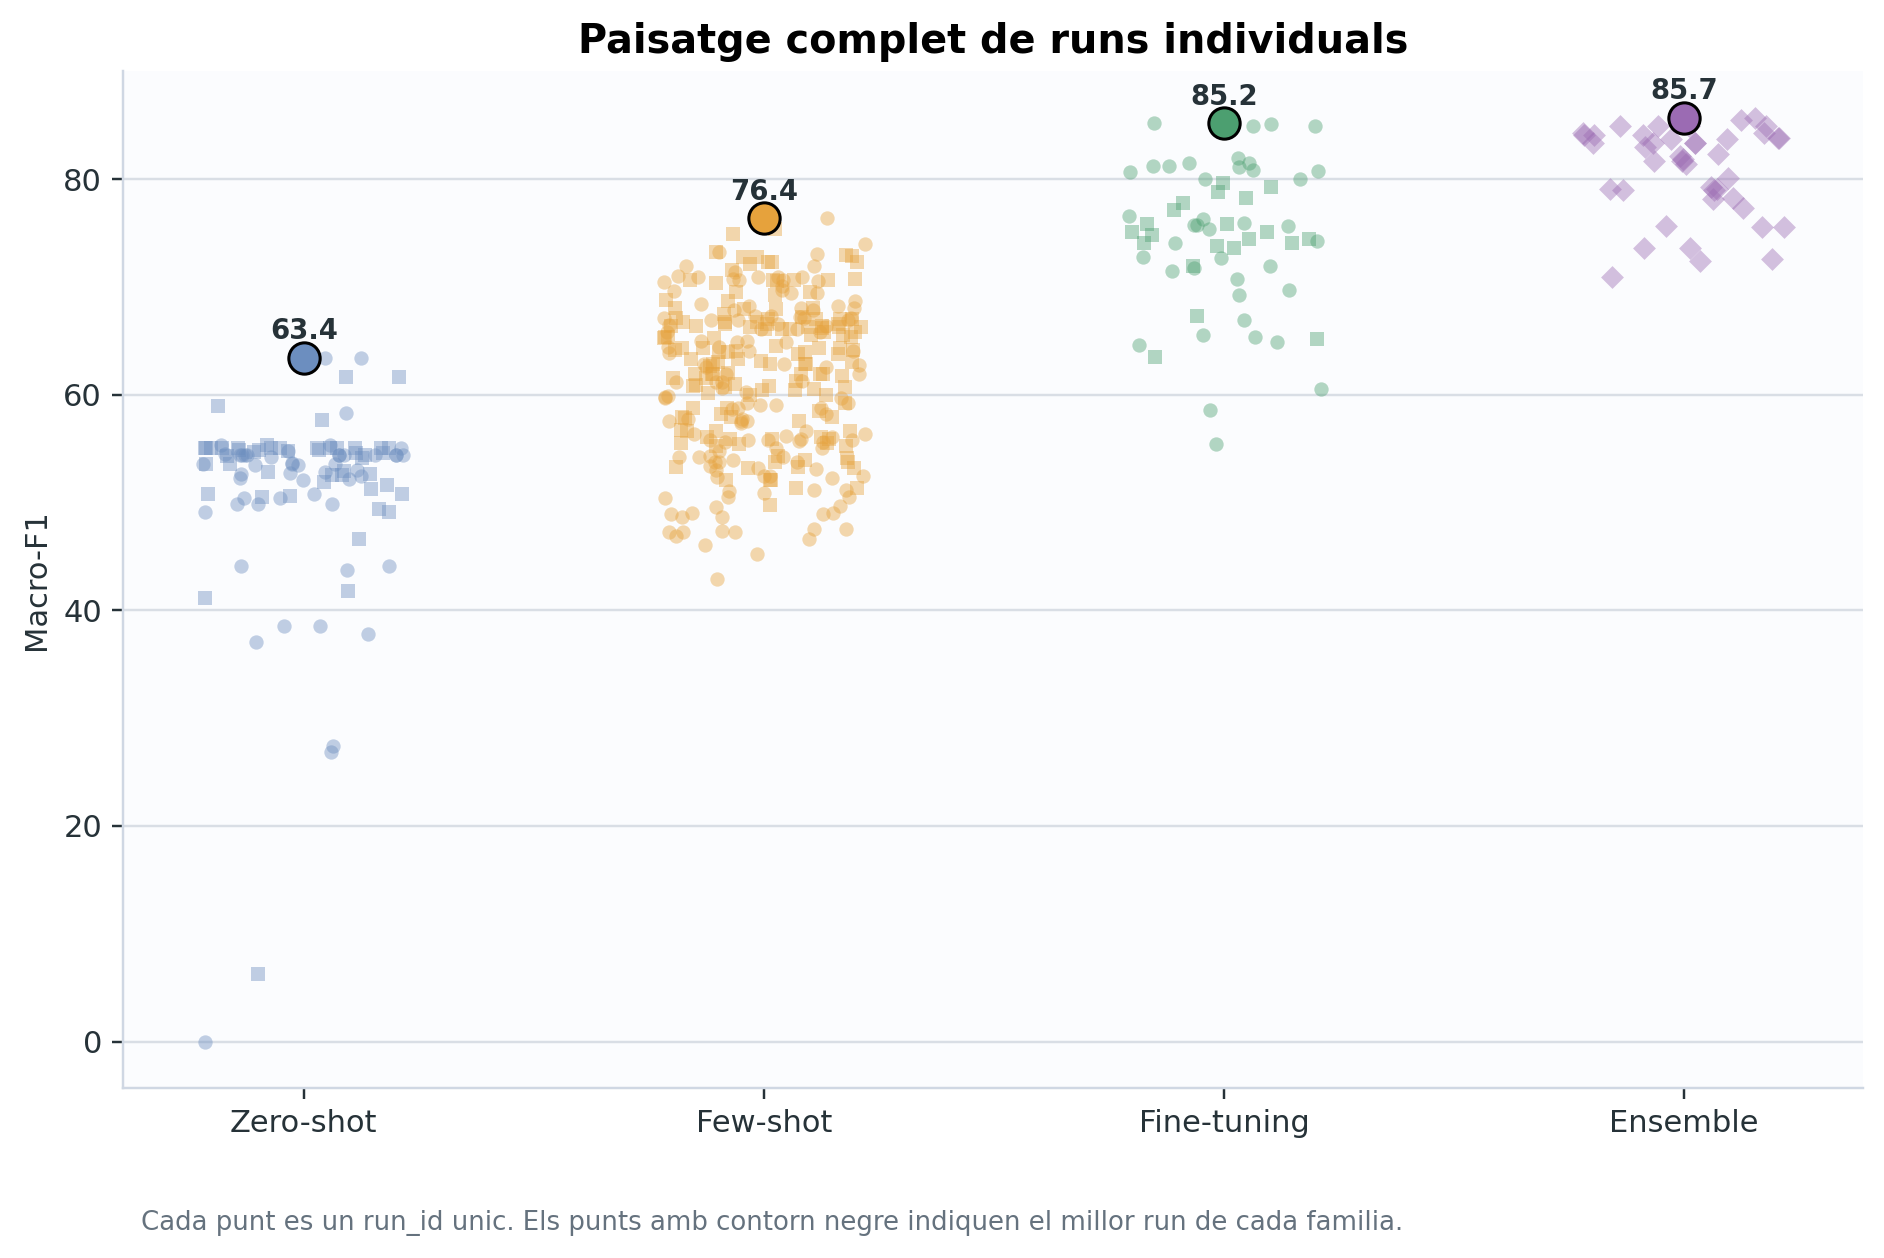
\includegraphics[width=\linewidth]{reports/report_assets/figures/00_run_landscape_individual_runs.png}
\caption{Paisatge complet de les execucions individuals. Cada punt correspon a un \texttt{run\_id} unic; els punts ressaltats indiquen el millor resultat de cada familia experimental.}
\label{fig:run-landscape}
\end{figure}

\input{reports/report_assets/tables/01_best_macro_f1_by_family.tex}

% ---------------------------------------------------------------------
% Zero-shot
% ---------------------------------------------------------------------

\begin{figure}[H]
\centering
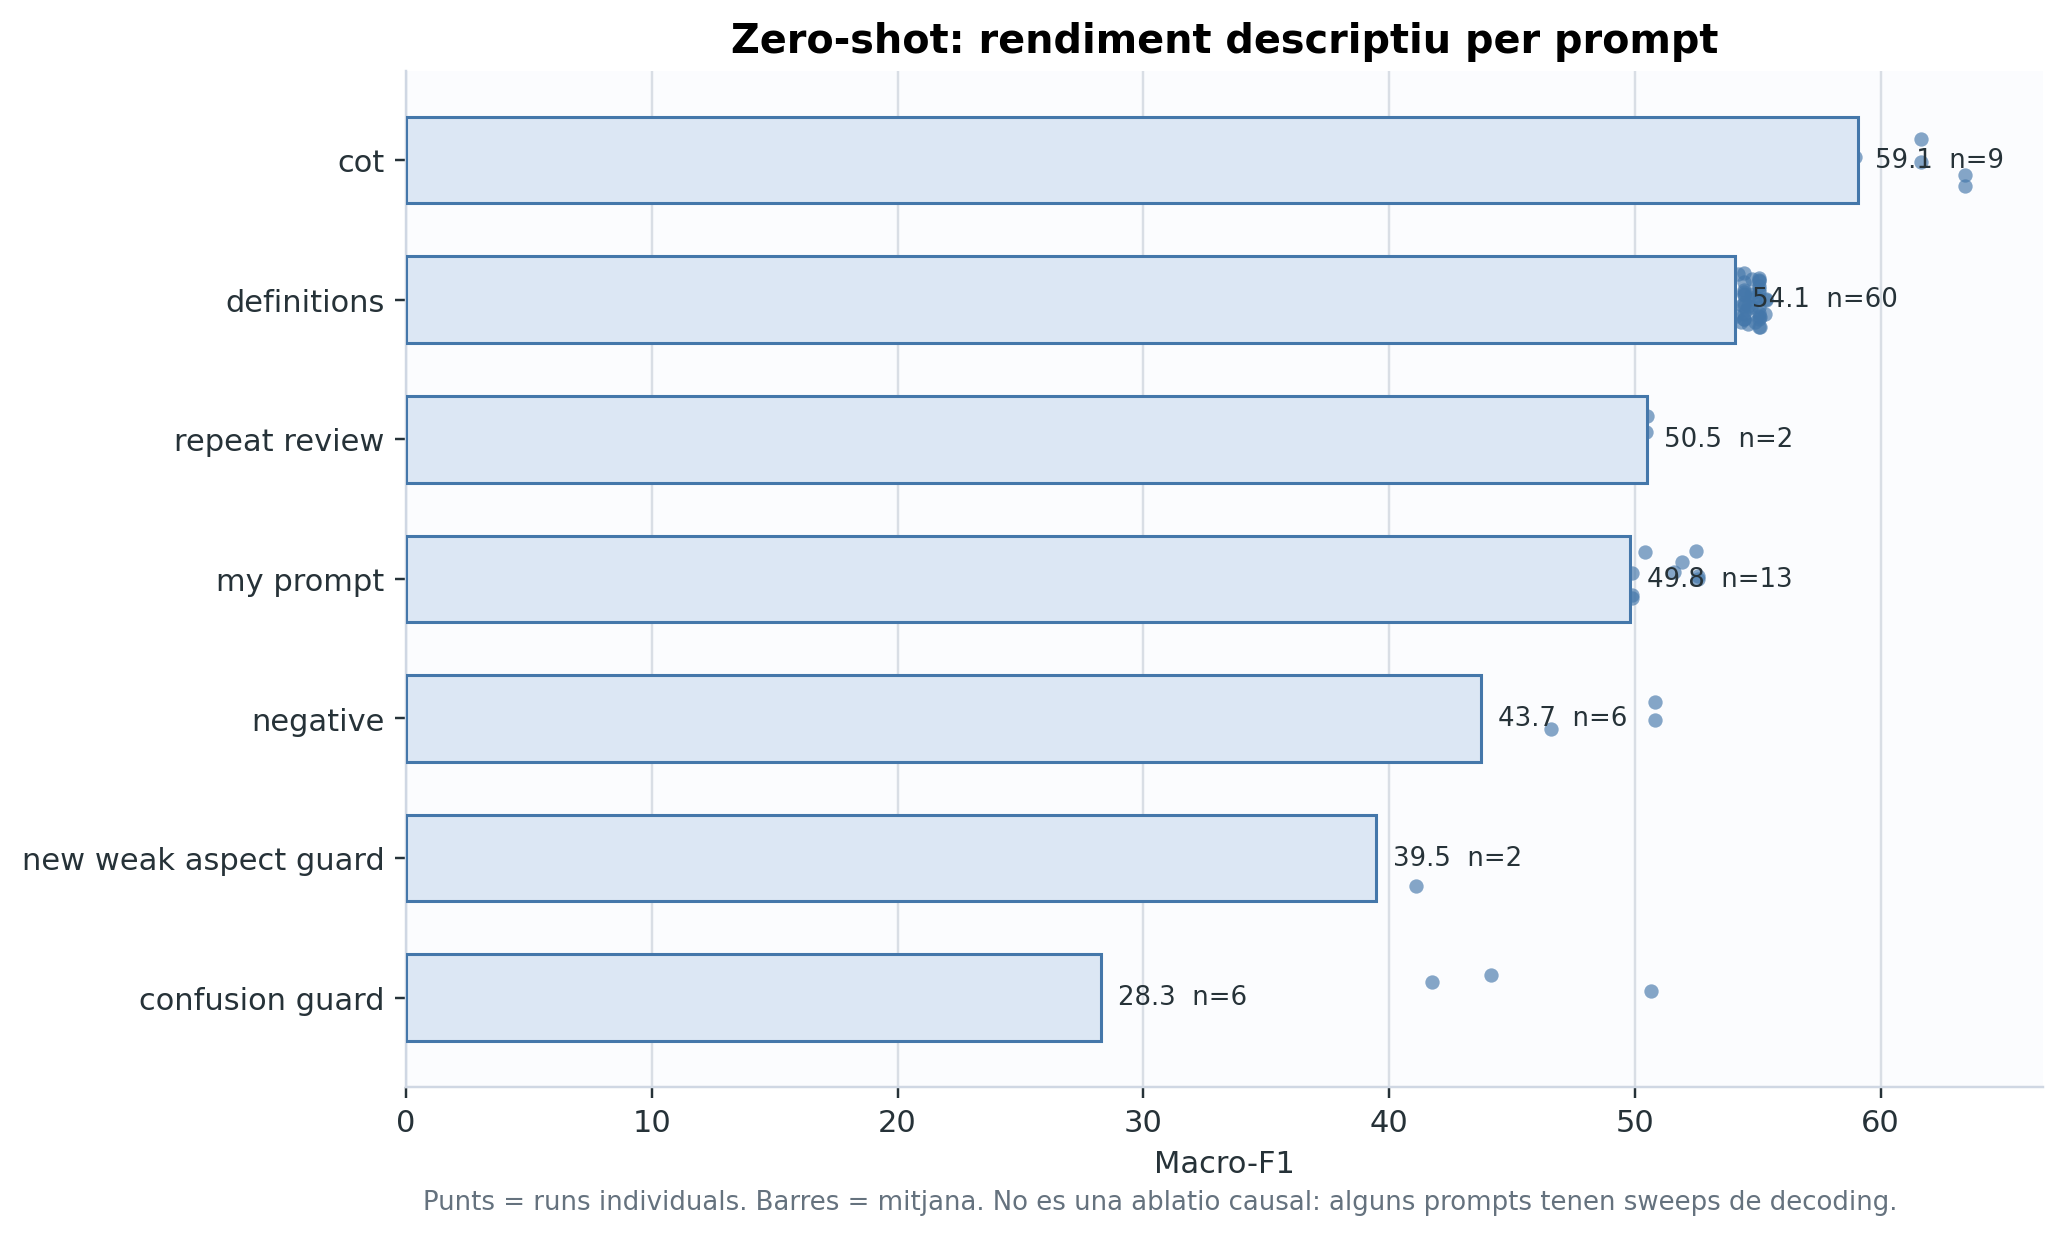
\includegraphics[width=\linewidth]{reports/report_assets/figures/02_zero_shot_prompt_descriptive.png}
\caption{Rendiment zero-shot per prompt. Aquesta figura es descriptiva: el prompt \texttt{definitions} inclou un sweep de decoding i, per tant, les conclusions causals s'han de basar en les comparacions aparellades.}
\label{fig:zero-prompt-descriptive}
\end{figure}

\input{reports/report_assets/tables/02b_zero_shot_controlled_deltas.tex}

\input{reports/report_assets/tables/03_zero_definitions_decoding.tex}

% ---------------------------------------------------------------------
% Few-shot
% ---------------------------------------------------------------------

\begin{figure}[H]
\centering
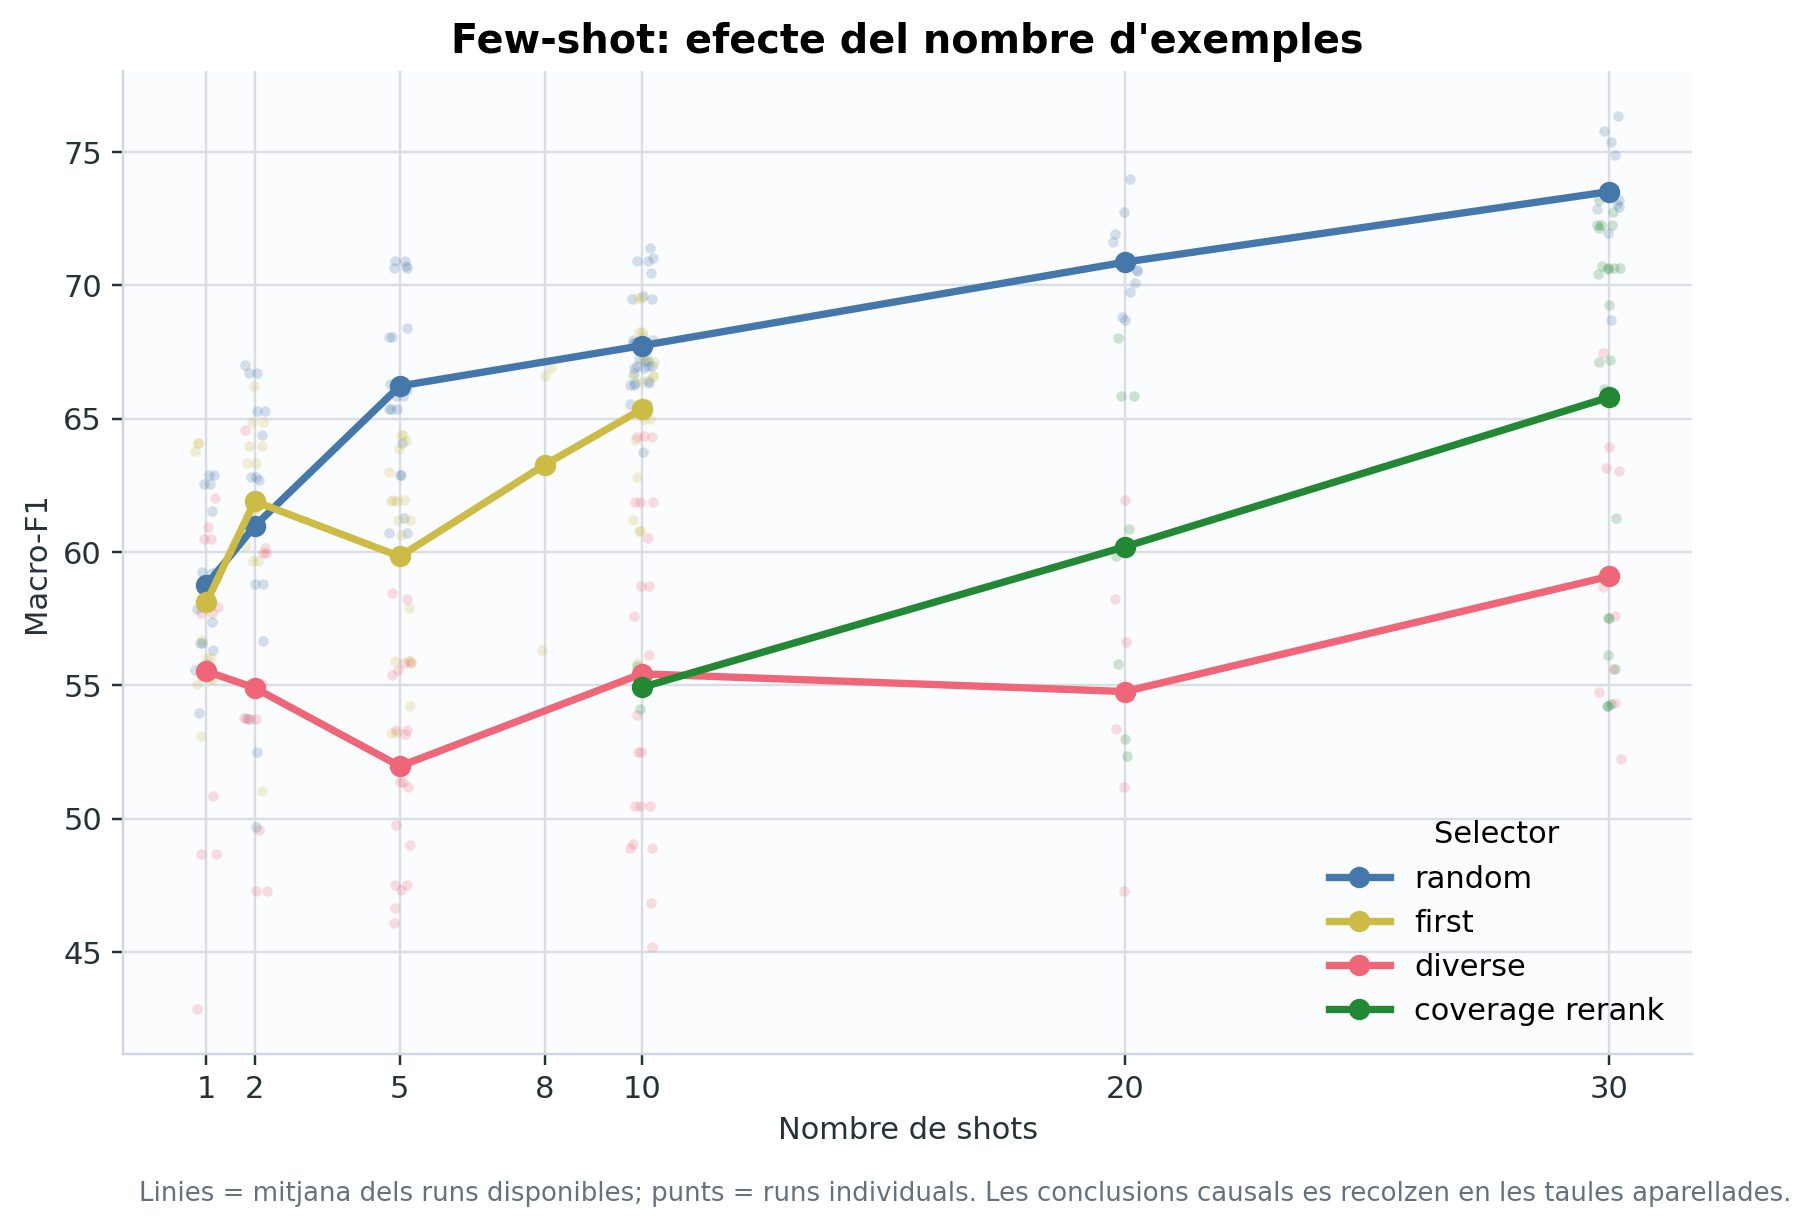
\includegraphics[width=\linewidth]{reports/report_assets/figures/04_few_shot_macro_by_shots_strategy.png}
\caption{Efecte del nombre de shots i de l'estrategia de seleccio en few-shot. Les linies son mitjanes dels runs disponibles i els punts mostren execucions individuals.}
\label{fig:few-shot-shots-strategy}
\end{figure}

\input{reports/report_assets/tables/04b_few_shot_controlled.tex}

\input{reports/report_assets/tables/04c_few_shot_shot_increments_random.tex}

% ---------------------------------------------------------------------
% Data augmentation
% ---------------------------------------------------------------------

\input{reports/report_assets/tables/05b_synthetic_dataset_audit.tex}

% ---------------------------------------------------------------------
% Fine-tuning
% ---------------------------------------------------------------------

\begin{figure}[H]
\centering
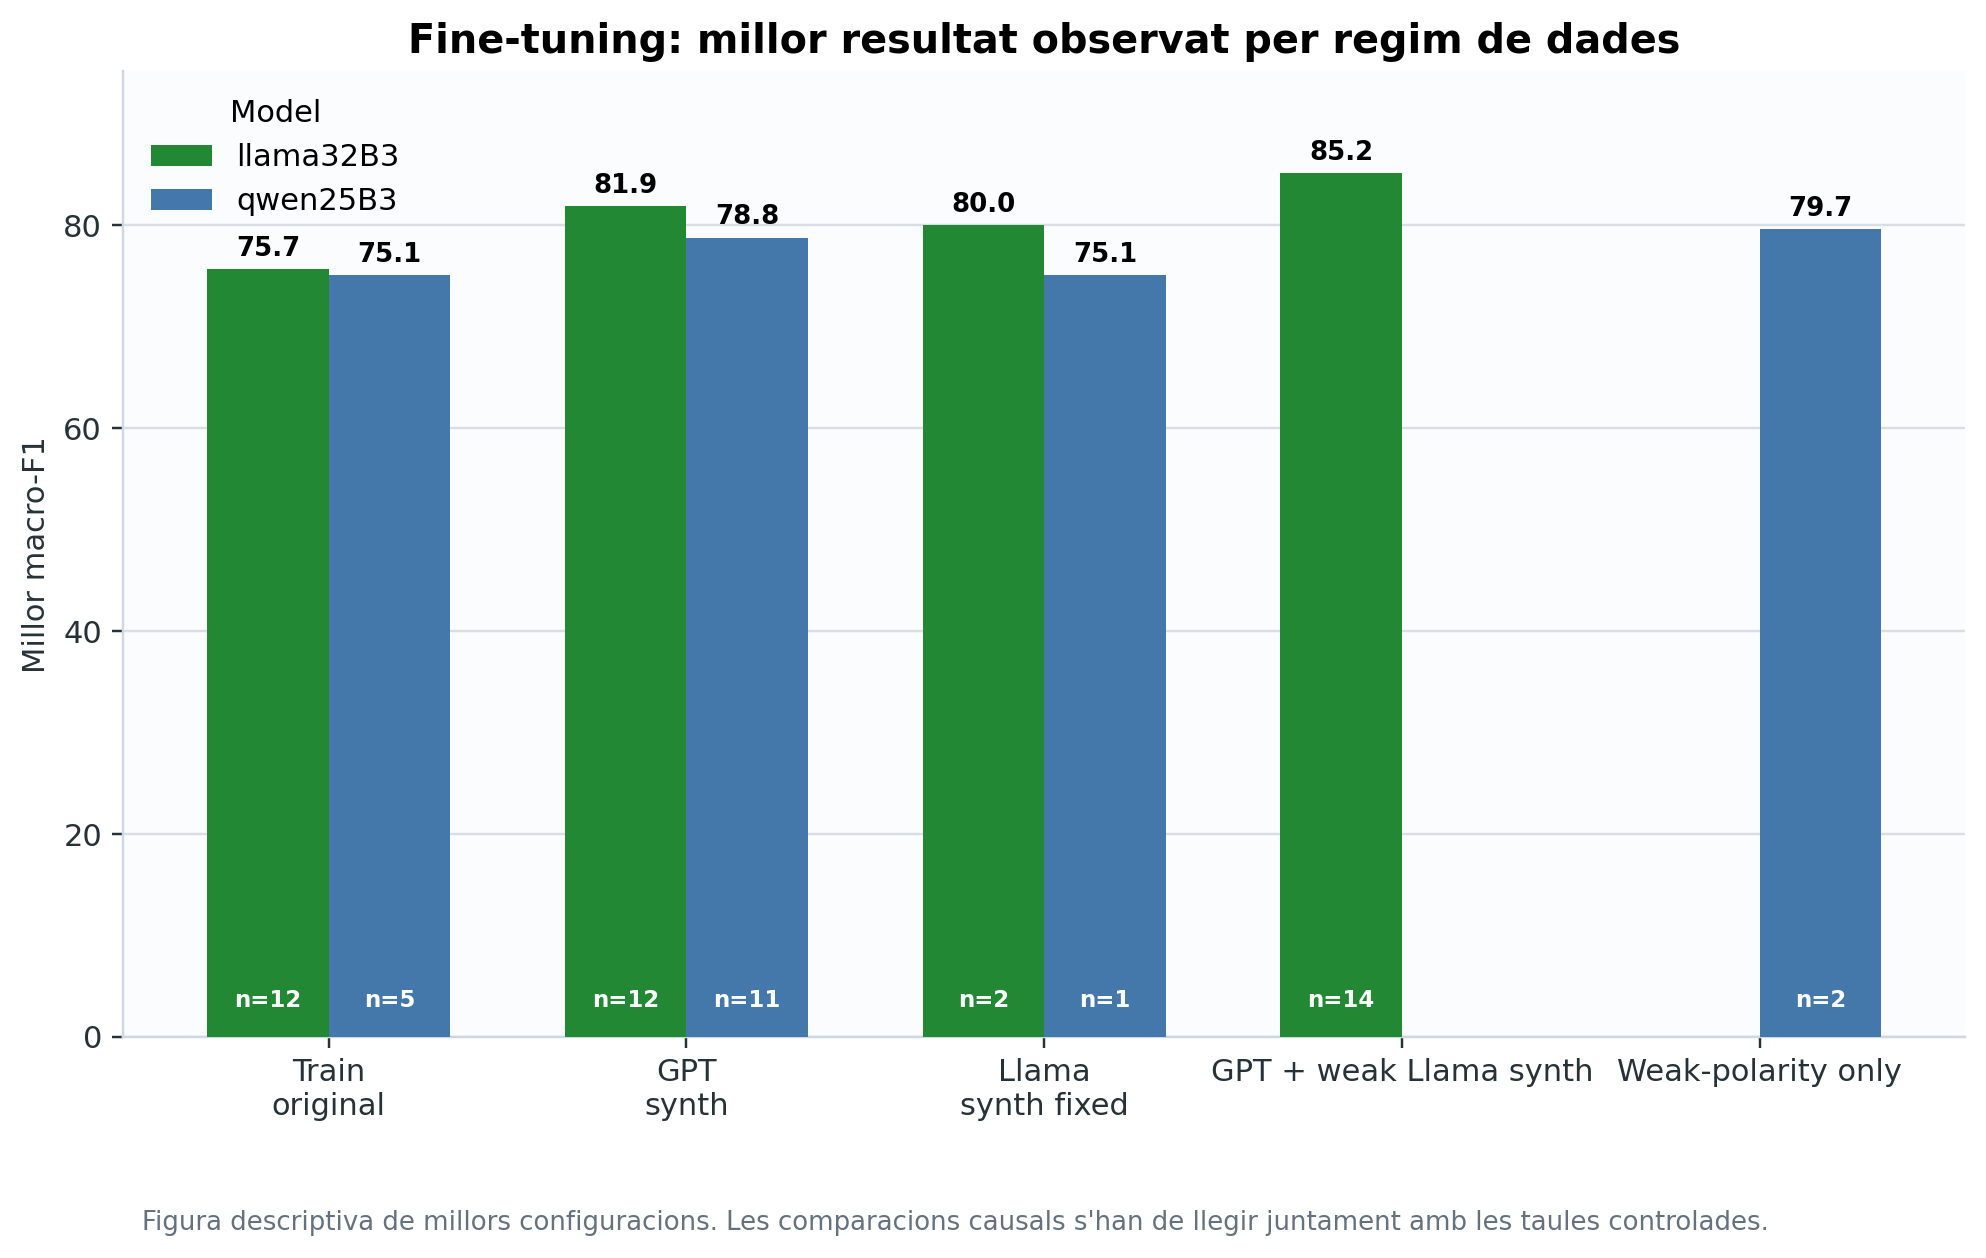
\includegraphics[width=\linewidth]{reports/report_assets/figures/06_finetune_best_by_data_regime.png}
\caption{Millor resultat observat per regim de dades i model en fine-tuning. Es una comparacio descriptiva: no totes les barres controlen exactament la resta d'hiperparametres.}
\label{fig:finetune-data-regime}
\end{figure}

\input{reports/report_assets/tables/06_finetune_best_by_data_regime.tex}

\begin{figure}[H]
\centering
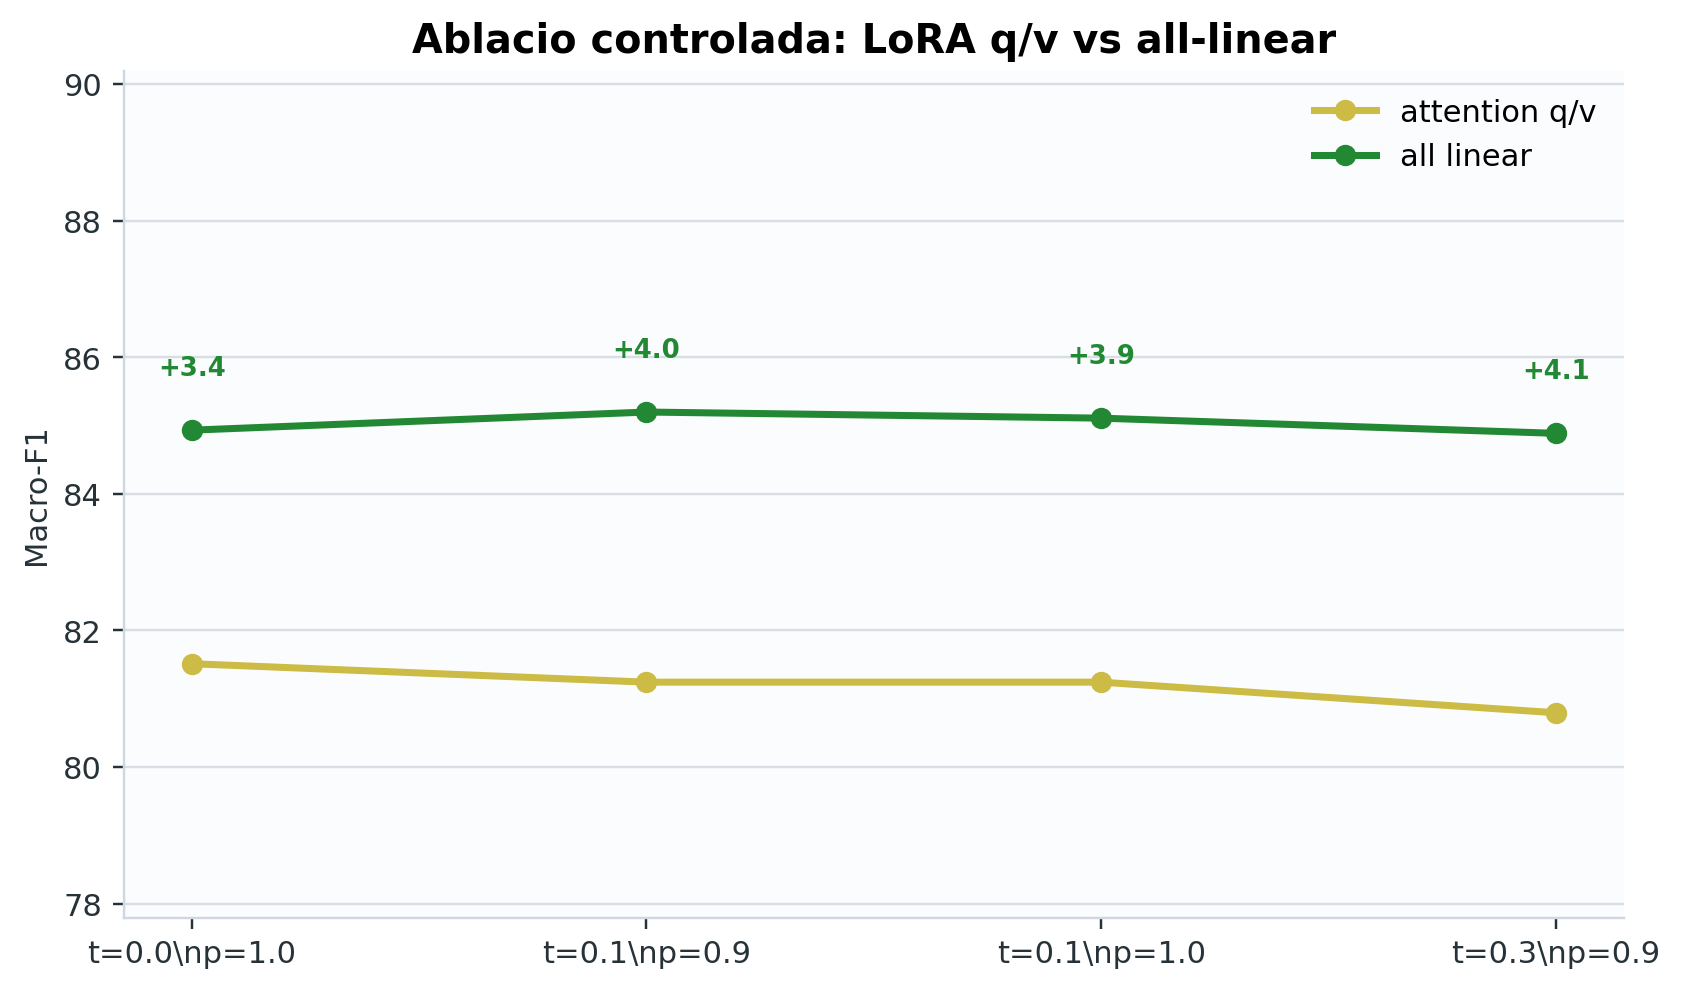
\includegraphics[width=0.88\linewidth]{reports/report_assets/figures/07_finetune_lora_target_controlled.png}
\caption{Ablacio controlada dels moduls LoRA en el millor regim Llama. Aplicar LoRA a totes les capes lineals supera de forma consistent la variant attention q/v.}
\label{fig:finetune-lora-target}
\end{figure}

\input{reports/report_assets/tables/07_finetune_lora_target_controlled.tex}

\begin{figure}[H]
\centering
\includegraphics[width=0.82\linewidth]{reports/report_assets/figures/07b_finetune_best_decoding.png}
\caption{Sweep de decoding sobre el millor adaptador fine-tuned. La millor macro-F1 apareix amb temperatura 0.1 i top-p 0.9, tot i que greedy decoding queda molt a prop.}
\label{fig:finetune-decoding}
\end{figure}

\input{reports/report_assets/tables/07b_finetune_best_decoding.tex}

\input{reports/report_assets/tables/12b_best_finetune_provenance_short.tex}

% ---------------------------------------------------------------------
% Ensembles
% ---------------------------------------------------------------------

\begin{figure}[H]
\centering
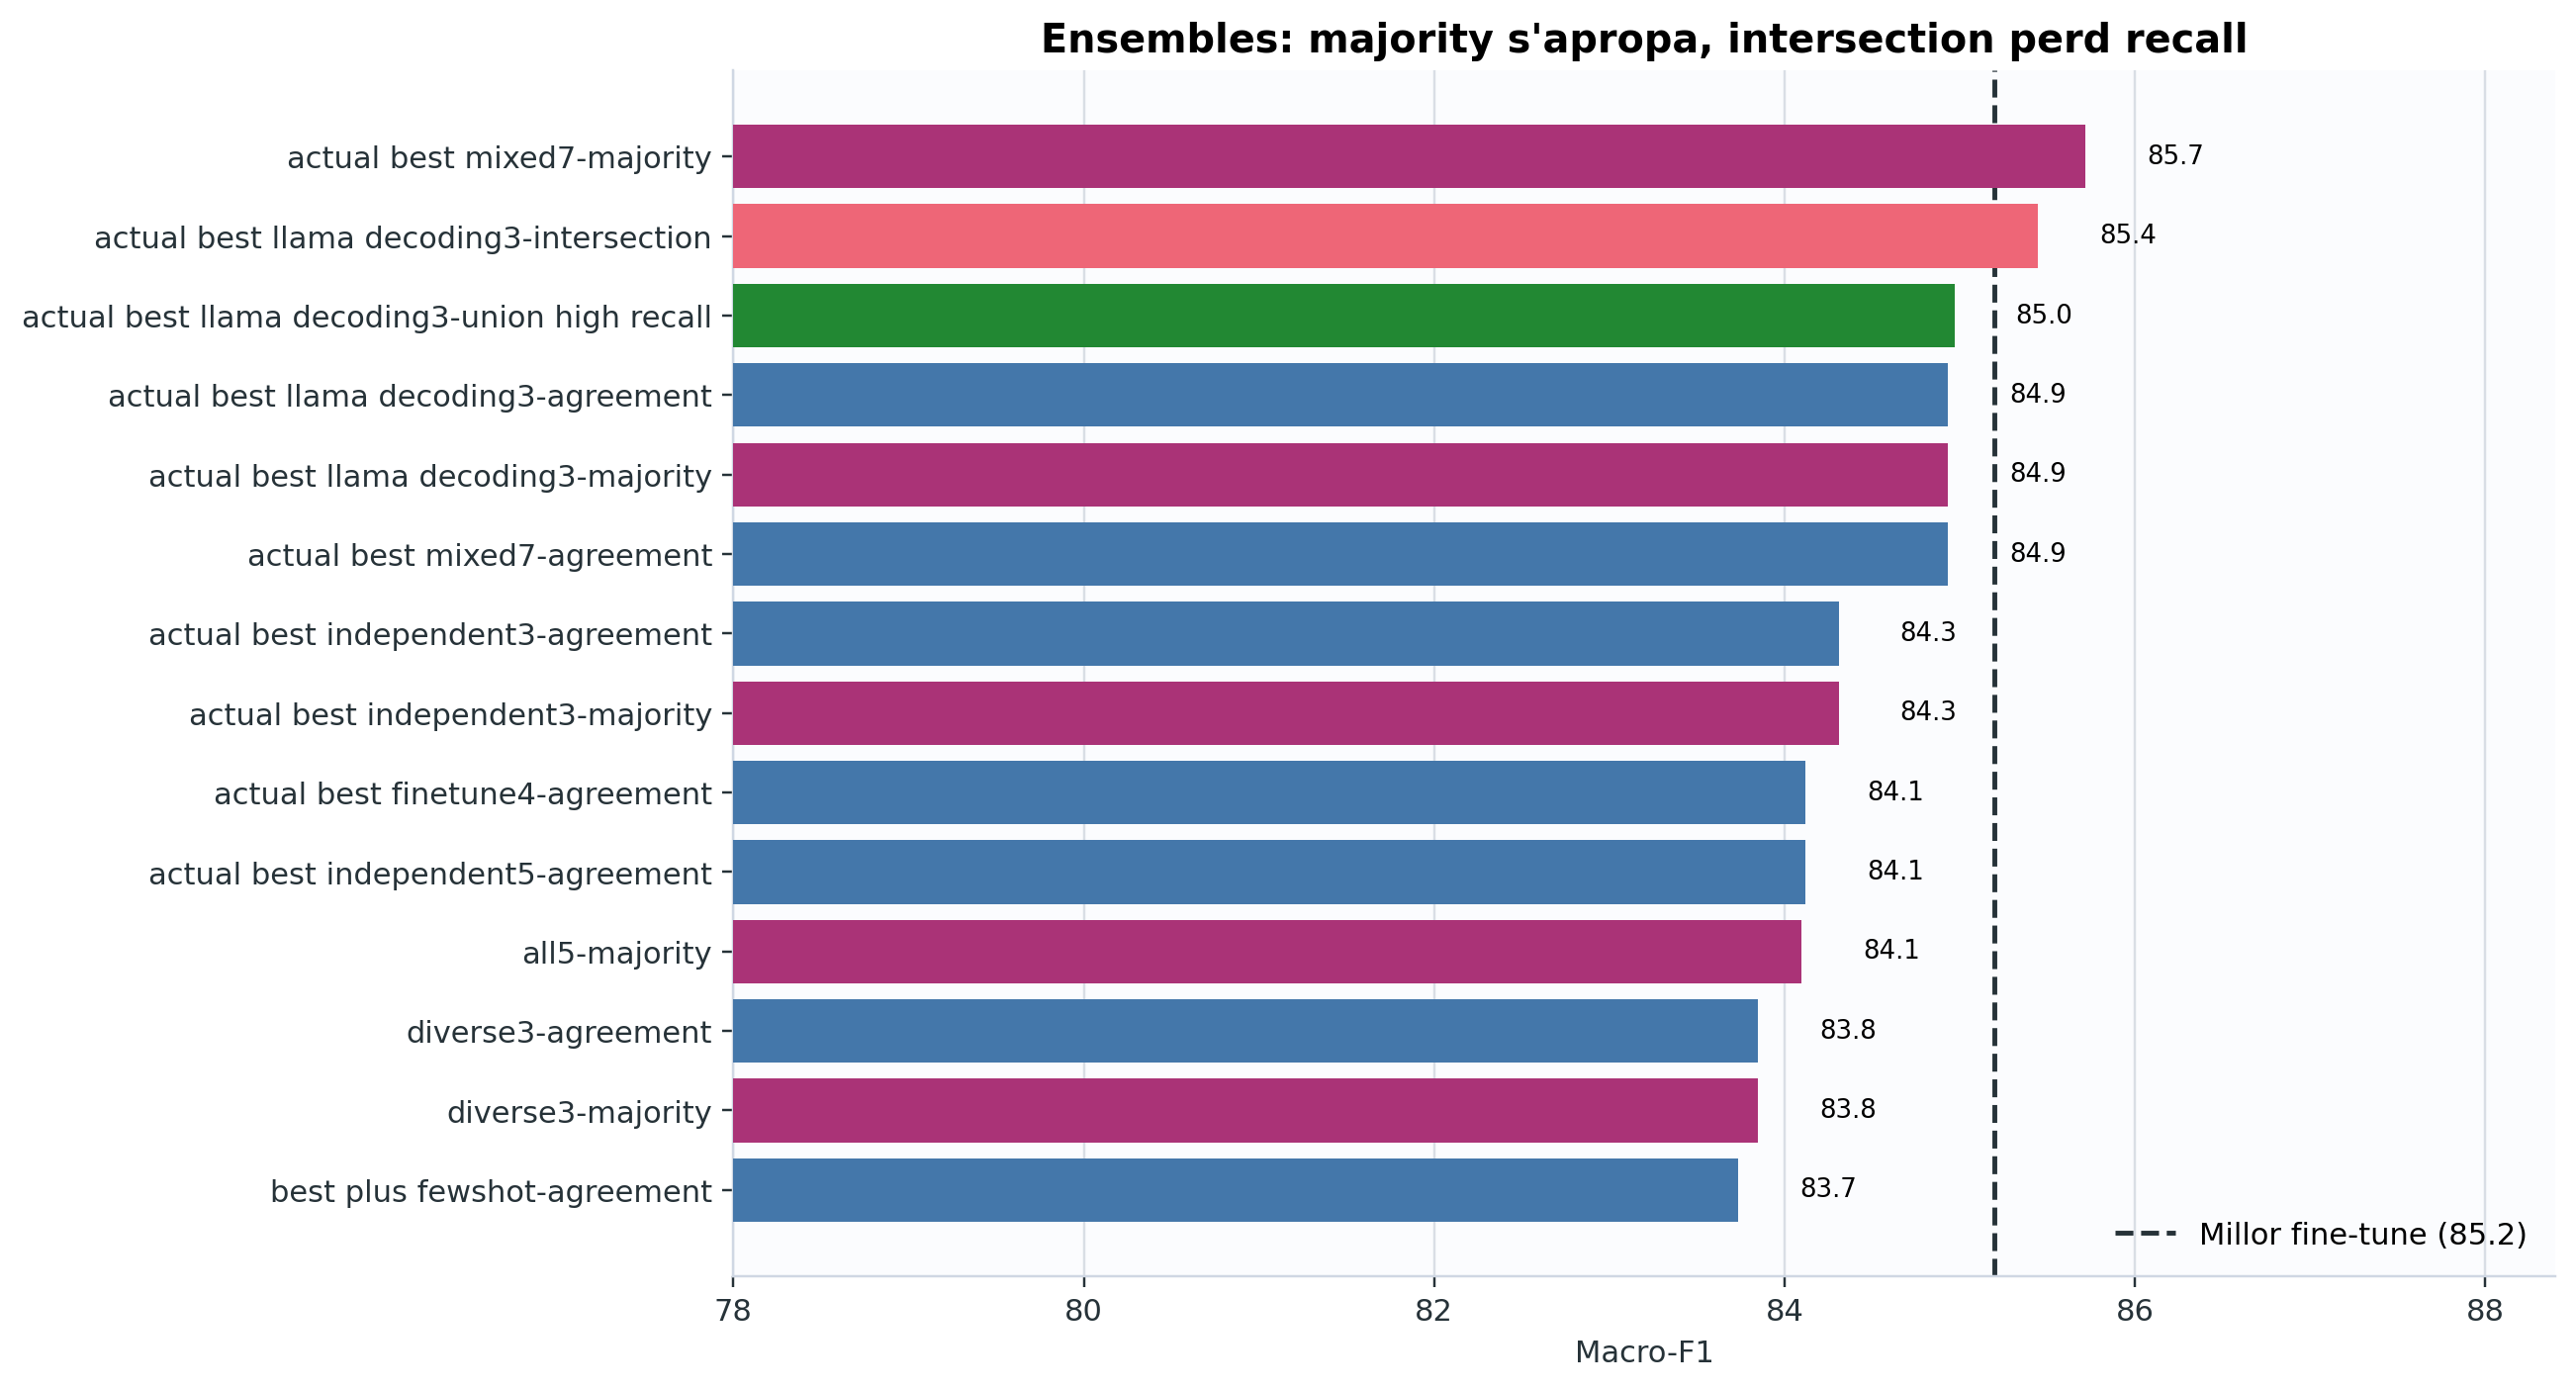
\includegraphics[width=\linewidth]{reports/report_assets/figures/08_ensemble_comparison.png}
\caption{Comparacio dels millors ensembles. La linia discontinua marca el millor fine-tune individual; el millor ensemble el supera lleugerament.}
\label{fig:ensemble-comparison}
\end{figure}

\input{reports/report_assets/tables/08_ensemble_comparison.tex}

\input{reports/report_assets/tables/08b_best_ensemble_members.tex}

% ---------------------------------------------------------------------
% Error analysis
% ---------------------------------------------------------------------

\begin{figure}[H]
\centering
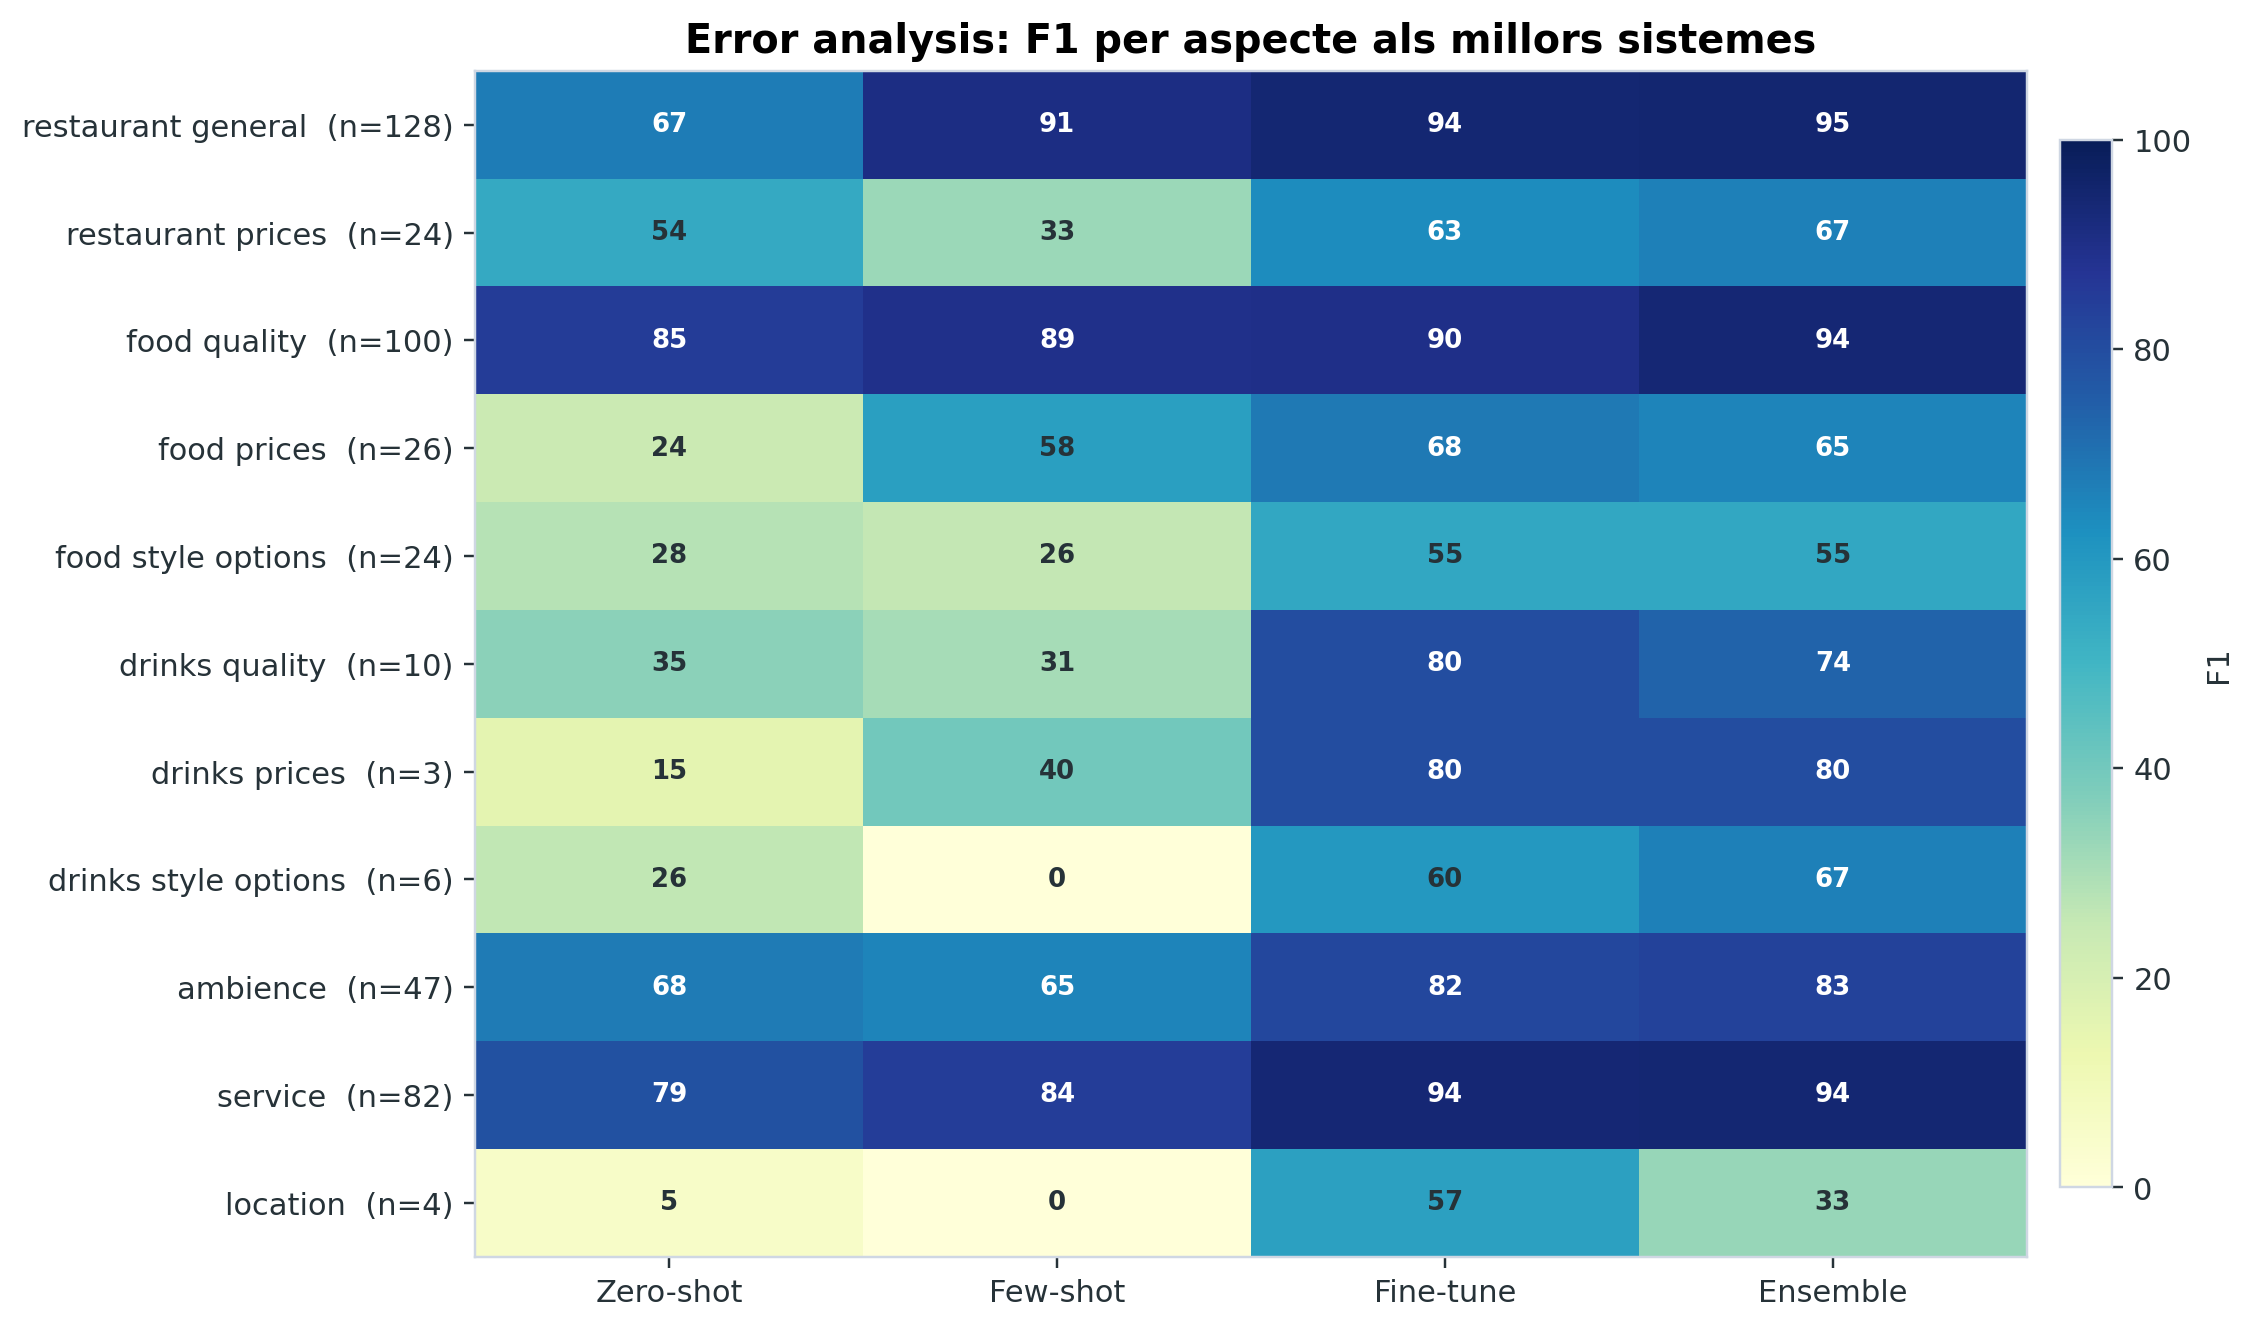
\includegraphics[width=\linewidth]{reports/report_assets/figures/09_error_analysis_per_aspect_heatmap.png}
\caption{F1 per aspecte als millors sistemes de cada familia. Els valors mostren que el fine-tuning millora sobretot classes minoritaries com \texttt{drinks\_quality}, \texttt{drinks\_prices} i \texttt{location}, encara que algunes continuen sent dificils.}
\label{fig:error-analysis-aspect}
\end{figure}

\input{reports/report_assets/tables/09_error_analysis_per_aspect.tex}

\begin{figure}[H]
\centering
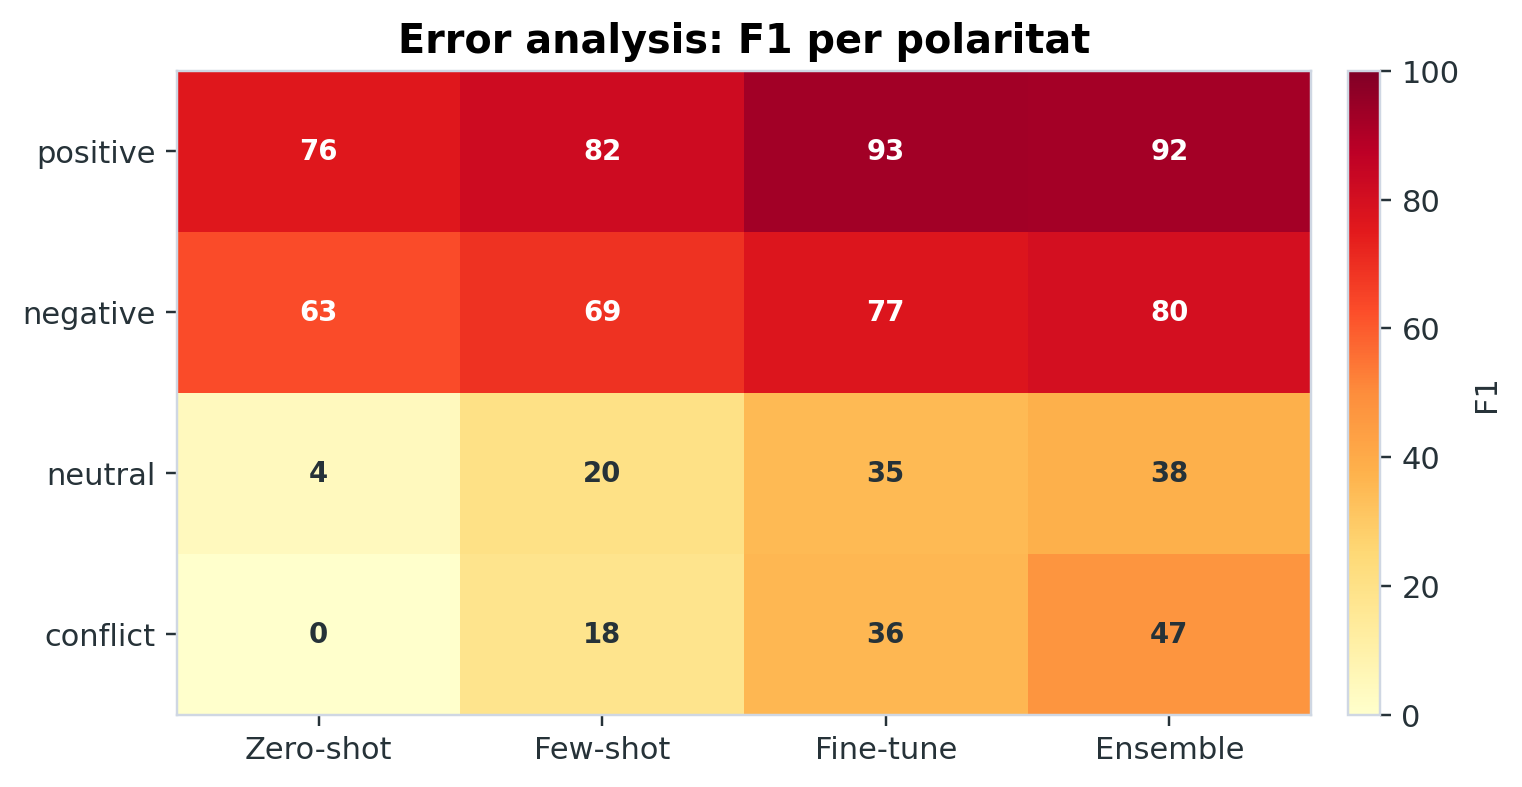
\includegraphics[width=0.82\linewidth]{reports/report_assets/figures/10_error_analysis_per_polarity_heatmap.png}
\caption{F1 per polaritat als millors sistemes. Les polaritats \texttt{neutral} i \texttt{conflict} continuen sent les mes dificils, tot i millorar clarament amb fine-tuning i ensemble.}
\label{fig:error-analysis-polarity}
\end{figure}

\input{reports/report_assets/tables/10_error_analysis_per_polarity.tex}
